\chapter{Mapeamento e diagrama arquitetural}
\label{cap:diagramas}

\section{Hierarquia de memória}
O sistema de memória de dados modelado com base no Intel i7 consiste em uma cache L1 de 32 KiB, com latência de acesso de quatro ciclos. A cache L2 (compartilhada com instruções) é de 256 KiB, com uma latência de acesso de 10 ciclos de \textit{clock}. A cache L3 tem 2 MiB e uma latência de acesso de 36 ciclos. Todas as caches são associativas por conjunto de oito vias e têm tamanho de bloco de 64 bytes. Permitir um acerto sob falta reduz a penalidade de falta em 9\% para os \textit{benchmarks} inteiros e de 12,5\% para os de ponto flutuante. Permitir um segundo acerto melhora esses resultados para 10\% e 16\%, e permitir 64 resulta em pouca melhoria adicional \cite{hennessy2019}.

\section{Divisão do endereço}
As caches possuem uma \textit{tag} de endereço em cada \textit{frame} de bloco, que indica o endereço do bloco. A \textit{tag} de cada bloco da cache que poderia conter a informação desejada é verificada, para saber se corresponde ao endereço de bloco do processador. Em geral, todas as \textit{tags} possíveis são pesquisadas em paralelo, pois a velocidade é crítica.

É preciso haver um meio de saber que um bloco de cache não tem informação válida. O procedimento mais comum é acrescentar um bit de validade à \textit{tag} para dizer se essa entrada contém ou não um endereço válido. Se o bit não for definido, não poderá haver uma combinação nesse endereço.

Antes de passar à próxima pergunta, vamos explorar o relacionamento de um endereço do processador com a cache. A primeira divisão ocorre entre o endereço de bloco e o \textit{offset} de bloco. O endereço do \textit{frame} de bloco pode ser dividido ainda mais, em campo de \textit{tag} e campo de índice. O campo de \textit{offset} de bloco seleciona os dados desejados do bloco, o campo de índice seleciona o conjunto e o campo de \textit{tag} é comparado com ele para ver se há um acerto. Embora a comparação pudesse ser feita sobre mais de um endereço do que a \textit{tag}, isso não é necessário, devido ao seguinte:
\begin{itemize}
    \item O \textit{offset} não deve ser usado na comparação, pois ou o bloco inteiro está presente ou não, e por isso todos os \textit{offsets} de bloco resultam em uma combinação por definição.
    \item A verificação do índice é redundante, pois foi usada para selecionar o conjunto a ser verificado. Um endereço armazenado no conjunto 0, por exemplo, precisa ter 0 no campo de índice ou não poderia ser armazenado no conjunto 0; o conjunto 1 precisa ter um valor de índice igual a 1, e assim por diante. Essa otimização economiza hardware e energia, reduzindo o tamanho da memória para a \textit{tag} de cache.
\end{itemize}

\begin{table}[H]
    \centering
    \begin{tabular}{|l|l|l|}
        \hline
        \multicolumn{2}{|c|}{Endereço de bloco} & \multirow{2}{*}{Offset de bloco} \\ \cline{1-2}
        Tag & Índice & \\ \hline
    \end{tabular}
    \caption{As três partes de um endereço em uma cache associativa em conjunto ou com mapeamento direto.}
    \label{tab:endereco}
    \fonte{Elaborado pelos autores (2026).}
\end{table}

A \textit{tag} é usada para verificar todos os blocos no conjunto, e o índice é usado para selecionar o conjunto. O \textit{offset} de bloco é o endereço dos dados desejados dentro do bloco. As caches totalmente associativas não possuem campo de índice.

Se o tamanho total da cache for mantido igual, o aumento da associatividade aumentará o número de blocos por conjunto, diminuindo assim o tamanho do índice e aumentando o tamanho da \textit{tag}. Ou seja, o limite de índice de \textit{tag} se move para a direita aumentando-se a associatividade, com a extremidade das caches totalmente associativas não possuindo campo de índice \cite{hennessy2019}.

\section{Esquema de cada mapeamento}
Podemos pensar em cada estratégia de posicionamento de bloco como uma variação da associatividade por conjunto. Uma cache diretamente mapeada é simplesmente uma cache associativa por conjunto de uma via: cada entrada de cache contém um bloco, e cada conjunto possui um elemento. Uma cache totalmente associativa com m entradas é simplesmente uma cache associativa por conjunto de m vias; ele tem um conjunto com m blocos, e uma entrada pode residir em qualquer bloco dentro desse conjunto. O tamanho total da cache em blocos é igual ao número de conjuntos multiplicado pela associatividade. Portanto, para uma cache de tamanho fixo, aumentar a associatividade diminui o número de conjuntos enquanto aumenta o número de elementos por conjunto \cite{hennessy2017}.

\begin{figure}[H]
    \centering
    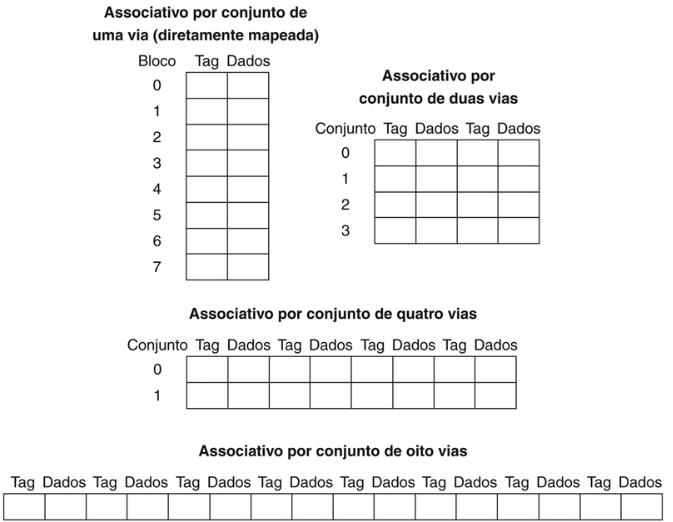
\includegraphics[width=0.9\textwidth]{figuras/endereco.png}
    \caption{Esquemas de mapeamento de cache}
    \label{fig:mapeamentos}
    \fonte{Elaborado pelos autores (2026).}
\end{figure}

\section{Fluxo de acesso à cache}
A \textit{tag} da cache é comparada com a parte superior do endereço para determinar se a entrada na cache corresponde ao endereço requisitado. Como a cache tem \(2^{10}\) (ou 1024) palavras e um tamanho de bloco de 1 palavra, 10 bits são usados para indexar a cache, deixando \(32 - 10 - 2 = 20\) bits para serem comparados com a \textit{tag}. Se a \textit{tag} e os 20 bits superiores do endereço forem iguais e o bit de validade estiver ligado, então, a requisição é um acerto na cache e a palavra é fornecida para o processador. Caso contrário, ocorre uma falha.

A unidade de controle precisa detectar uma falha de cache e processá-la buscando os dados requisitados da memória (ou, como veremos, de uma cache de nível inferior). Se a cache reportar um acerto, o computador continua usando os dados como se nada tivesse acontecido \cite{patterson2017}.

\section{Cache da máquina usada na PoC}
\label{sec:cache-poc}
A máquina utilizada para os testes da PoC possui um processador Intel Core i5-12500H (12ª geração) e sistema operacional Fedora Linux. De acordo com o comando \texttt{lscpu}, a hierarquia de cache é composta por 448 KiB de cache L1 de dados (L1d), 640 KiB de cache L1 de instruções (L1i), 9 MiB de cache L2 e 18 MiB de cache L3 compartilhada.